% Pre-warms the offline Tectonic cache baked into the compiler image. The runtime compiles with
% --only-cached and has no network access, so every package, TikZ library, font shape/size and
% bundled graphic (example-image) the TikzForge serializer can emit must be exercised here. The
% preamble must match PICTURE_PREAMBLE in crates/tikz-serializer/src/lib.rs.
\documentclass{standalone}
\usepackage{tikz}
\usepackage{pgfplots}
\pgfplotsset{compat=1.18}
\usepackage{amsmath}
\usepackage{amssymb}
\usetikzlibrary{arrows.meta,calc,positioning,shapes.geometric,fit,backgrounds}
\begin{document}
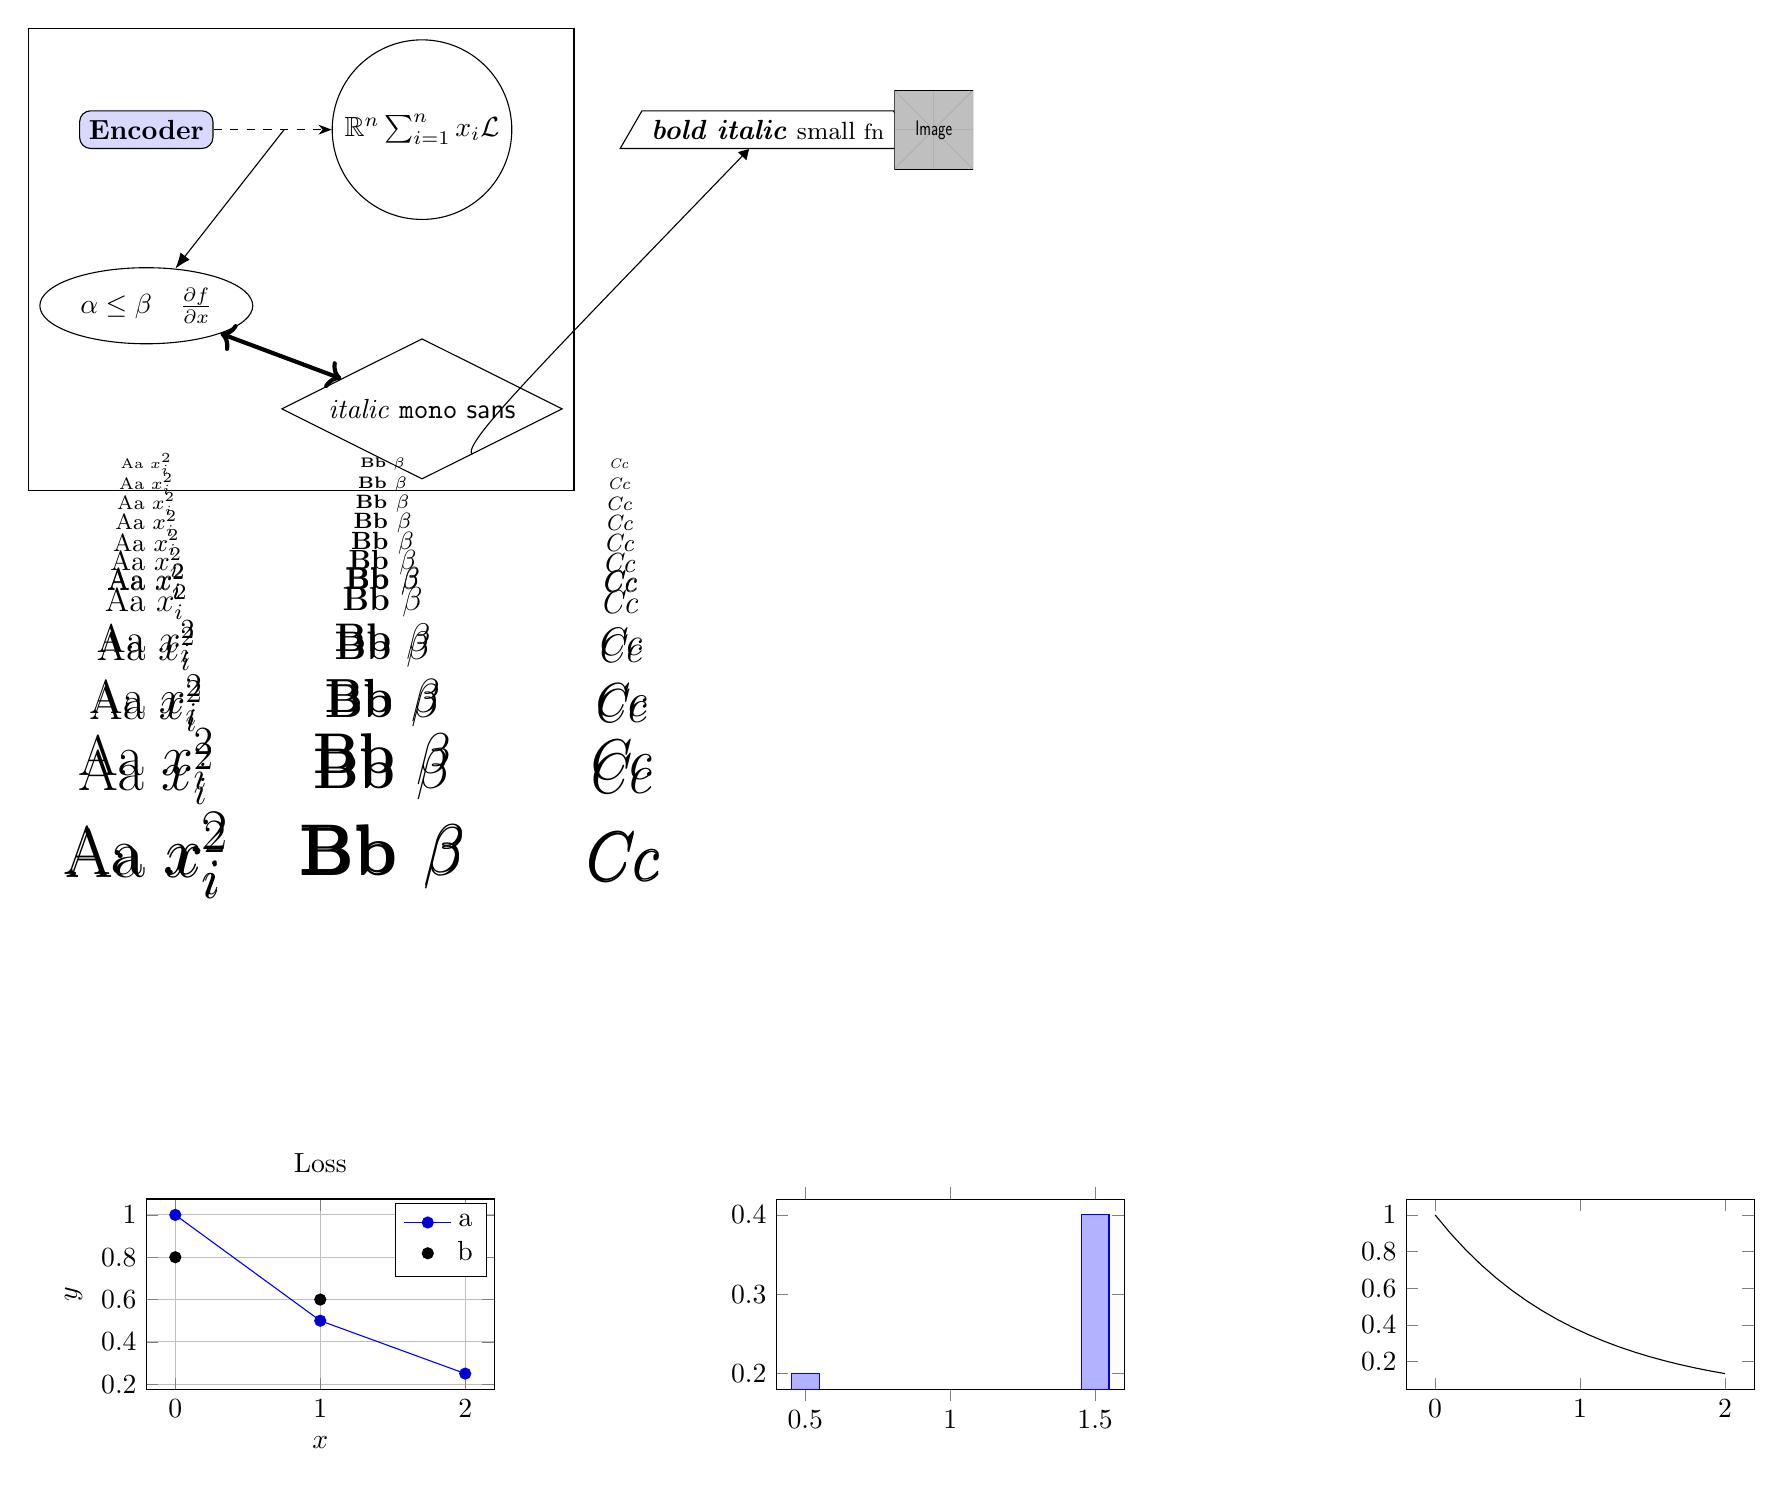
\begin{tikzpicture}[node distance=1.5cm]
  \node[draw, rounded corners, fill=blue!15, font=\bfseries] (a) {Encoder};
  \node[draw, circle, right=of a] (b) {$\mathbb{R}^{n}\sum_{i=1}^{n} x_i \mathcal{L}$};
  \node[draw, ellipse, below=of a] (c) {$\alpha \leq \beta \quad \frac{\partial f}{\partial x}$};
  \node[draw, diamond, aspect=2, below=of b] (d) {\textit{italic} \texttt{mono} \textsf{sans}};
  \node[draw, trapezium, right=of b] (e) {\textbf{\textit{bold italic}} \small small \footnotesize fn};
  \draw[-Stealth, dashed] (a) -- (b);
  \draw[-{Latex[length=2mm]}] ($(a)!0.5!(b)$) -- (c);
  \draw[<->, line width=1.5pt] (c) -- (d);
  \draw[-Triangle] (d) .. controls (4,-4) and (5,-3) .. (e);
  \begin{scope}[on background layer]
    \node[draw, fit=(a)(b)(c)(d), inner sep=4pt] {};
  \end{scope}
  % Image nodes default to mwe's placeholder until the user uploads a file.
  \node[inner sep=0pt] at (10,0) {\includegraphics[width=1cm,height=1cm]{example-image}};
  \foreach \size in {5,6,7,8,9,10,10.95,11,12,14,14.4,17,17.28,20,20.74,24.88,25} {
    \node[font=\fontsize{\size pt}{\size pt}\selectfont] at (0,-3-\size/4) {Aa $x^2_{i}$};
    \node[font=\bfseries\fontsize{\size pt}{\size pt}\selectfont] at (3,-3-\size/4) {Bb $\beta$};
    \node[font=\itshape\fontsize{\size pt}{\size pt}\selectfont] at (6,-3-\size/4) {Cc};
  }
  \begin{axis}[at={(0,-16cm)}, width=6cm, height=4cm, title={Loss}, xlabel={$x$}, ylabel={$y$},
      legend entries={a,b}, grid=major]
    \addplot coordinates {(0,1) (1,0.5) (2,0.25)};
    \addplot[only marks] coordinates {(0,0.8) (1,0.6)};
  \end{axis}
  \begin{axis}[at={(8cm,-16cm)}, ybar, width=6cm, height=4cm]
    \addplot coordinates {(0.5,0.2) (1.5,0.4)};
  \end{axis}
  \begin{axis}[at={(16cm,-16cm)}, width=6cm, height=4cm]
    \addplot[domain=0:2, samples=20] {exp(-x)};
  \end{axis}
\end{tikzpicture}
\end{document}
